\documentclass[fleqn]{jbook}
\usepackage{physpub}

\begin{document}
\begin{question}{教育 数学}{}

\begin{subquestions}
\SubQuestion
以下の設問に答えよ。
\begin{subsubquestions}
\SubSubQuestion
$\alpha$を実数としたときに次の積分を複素積分の方法を用いて求めよ。
\[ \int_{0}^{\infty} \d x \frac{\sin \alpha x}{x} \]

\SubSubQuestion
区間$[-\pi, \pi]$で定義された関数$f(x)=|x|$のフーリエ級数展開を次のように
表したとする:
\[ f(x) = \frac{a_0}{2} + \sum_{n=1}^{\infty} (a_n \cos nx + b_n \sin n x) 
\hspace{2cm} x \in [-\pi, \pi]\]
このとき$a_n (n=0,1,2,\cdots), b_n(n=1,2,\cdots)$を求め、
この結果を用いて、次式を証明せよ。
\[ 1 + \frac{1}{3^2} + \frac{1}{5^2} + \cdots = \sum_{n=0}^{\infty}
\frac{1}{(2n+1)^2} = \frac{\pi^2}{8}\]
\end{subsubquestions}

\SubQuestion
3行3列の実行列$A=\{ a_{ij} \}$が与えられているとき、行列式$\mbox{det} [ A-
\lambda I ]$はパラメータ$\lambda$について3次の多項式となる。ただし、$I$は
単位行列である。上の行列式を次のように書くことにする:
\[ F(\lambda) \equiv \mbox{det} [ A-\lambda I ] = -\lambda^3 + P \lambda ^2 
+ Q \lambda + R\]
このとき以下の設問に答えよ。

\begin{subsubquestions}
\SubSubQuestion
上の3次式の係数$P,Q,R$は次のように表せることを示せ。

\begin{eqnarray*}
P &=& \mbox{Tr} A \hspace{1cm}
Q = \frac{1}{2} \left( \mbox{Tr} A^2 - ( \mbox{Tr} A)^2 \right) \hspace{1cm}
R =\mbox{det} A
\end{eqnarray*}
ここで、$\mbox{Tr}$は行列の対角和を意味する。

\SubSubQuestion
特に$P=0$のとき、行列$A=\{ a_{ij} \}$が複素共役の固有値を持つための条件を
$Q,R$を使って表せ。

\end{subsubquestions}
\SubQuestion
$H_n(x)(n=0,1,2,\cdots)$を$x$の$n$次の多項式で次の性質を満たすものとする。

\[H_n(x)=x^n+(nより低次の多項式) \]
\[\int_{-\infty}^{\infty} \d x e^{-x^2} H_n (x) H_m (x) = 0 \hspace{1cm}
(n \neq m)\]
\begin{subsubquestions}

\SubSubQuestion
$n=1,2,3$について$H_n(x)$を具体的に構成せよ。ただし次の積分公式を
用いて良い。
\[ \int_{-\infty}^{\infty} \d x x^{2m} e^{-x^2} = \sqrt{\pi} \frac{(2m)!}{4^m
m!} \hspace{2cm} (m=0,1,2,\cdots)\]

一般に$n$次の多項式$P(x)$は$H_l(x)$を用いて$P(x)=\displaystyle{\sum_{l=0}^{n} c_l H_l (x)}$と展開できることを注意し、次の設問に答えよ。

\SubSubQuestion
$H_n(-x)-(-1)^n H_n(x) = 0$となることを帰納法を用いて証明せよ。

\SubSubQuestion
$a_n$を適当な係数として$H_n(x)$が次の形の漸化式を満たすことを証明せよ。
\begin{eqnarray*}
x H_n(x) &=& H_{n+1} (x) + a_n H_{n-1} (x) \\
\frac{\d}{\d x} H_n (x) &=& n H_{n-1} (x)
\end{eqnarray*}
\end{subsubquestions}
\end{subquestions}
\end{question}
\begin{answer}{教育 数学}{}
\begin{subanswers}
\SubAnswer
\begin{subsubanswers}
\SubSubAnswer
まず、$\alpha  = 0$のときは被積分関数は$0$なので明らかに
\[ \int_{0}^{\infty} \d x \frac{\sin \alpha x}{x} = 0.\]

次に被積分関数は偶関数であるから、
\[ \int_{0}^{\infty} \d x \frac{\sin \alpha x}{x} = \frac{1}{2} \int_{-\infty}
^{\infty} \d x \frac{\sin \alpha x}{x}.\]
\parbox[t]{110mm}{さらに、この積分は
\[ \mbox{Im} \left[ \frac{1}{2} \int_{-\infty}^{\infty} \d x
\frac{e^{i \alpha x}}{x} \right]\]
とかける。

そこで、この積分を図のような積分路で計算する。
積分路に囲まれた領域内には極は存在しないので、
\[ \int_{\text{C}} \frac{e^{i \alpha z}}{z} = 0.\] }
%%%%%%%%%%%%%%%%%%%%%%
\parbox[t]{60mm}{\vspace*{3mm}
\begin{center}
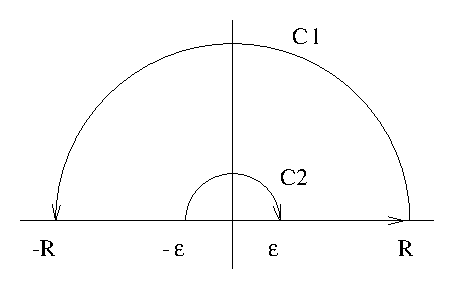
\includegraphics[clip,width=50mm]{1998math1.eps}
\end{center}
}
$ \alpha > 0$のときは上半面で計算する。

大きな円弧状では$ z= R e^{i \theta}$とかける。この時、
この円弧上の積分の寄与は
\begin{eqnarray*}
\left| \int_{\text{C}_1} \frac{e^{i \alpha z}}{z} \d z \right|&=&
\left| \int_{0}^{\pi} i R e^{i \theta} \d \theta \frac{e^{i \alpha R 
(\cos \theta + i \sin \theta)}}{ R e^{i \theta}} \right|
= \left|i \int_{0}^{\pi} \d \theta e^{-\alpha R \sin \theta} 
e^{i \alpha R \cos \theta} \right| \\
&\leq&  \int_{0}^{\pi} \d \theta e^{-\alpha R \sin \theta} 
\end{eqnarray*}
$\sin \theta$は、$\theta = \frac{\pi}{2}$で折り返し対称なので、
\begin{eqnarray*}
=2 \int_{0}^{\frac{\pi}{2}} \d \theta e^{-\alpha R \sin \theta} 
\leq 2 \int_{0}^{\frac{\pi}{2}} \d \theta e^{\frac{-2\alpha R \theta}{\pi}} 
=\frac{\pi}{\alpha R} (1-e^{-\alpha R}) \rightarrow 0
 \quad (R \rightarrow \infty)
\end{eqnarray*}

それゆえ、
\[ \int_{-R}^{-\varepsilon} \d x \frac{e^{i \alpha x}}{x}
+ \int_{\varepsilon}^{R} \d x \frac{e^{i \alpha x}}{x} 
+ \int_{\text{C}_2} \d z \frac{e^{i \alpha z}}{z} = 0.\]

この最後の項を計算する。$\mbox{C}_2$上では$z=\varepsilon e^{i \theta}$
であるから、この上では$\varepsilon$が微小だとすると
\begin{eqnarray*}
\int_{\text{C}_2} \frac{e^{i \alpha z}}{z} \d z &=& \int_{\pi}^{0}
\frac{e^{i \alpha \varepsilon e^{i \theta}}}{\varepsilon e^{i \theta}}
\varepsilon i e^{i \theta} \d \theta \\
&=& i \int_{\pi}^{0} \d \theta e^{i \alpha \varepsilon e^{i \theta}}
= i \int_{\pi}^{0} \left\{ 1 + i \alpha \varepsilon e^{i \theta}
+ {\cal{O}}(\varepsilon^2) \right\} \d \theta \\
&=& - i\pi.
\end{eqnarray*}

それゆえ、
\[ \int_{-R}^{-\varepsilon} + \int_{\varepsilon}^{R} \frac{e^{i\alpha x}}{x}
\d x = i \pi.\]
$R \rightarrow \infty, \varepsilon \rightarrow 0$として虚部をとると、
\[ \int_{0}^{\infty} \d x \frac{\sin \alpha x}{x} = \frac{\pi}{2}\]
を得る。

$\alpha <0$の場合、
\[ \int_{0}^{\infty} \d x \frac{\sin \alpha x}{x} = 
\int_{0}^{\infty} \d x \frac{-\sin \left| \alpha \right|x}{x} =
-\int_{0}^{\infty} \d x \frac{\sin \left| \alpha \right|x}{x} =
-\frac{\pi}{2}\]
を得る。

%%%%%%%%%%%%%%%%%%%%%%%%%%%%%%
\SubSubAnswer

まず、
\begin{eqnarray*}
\int_{-\pi}^{\pi} \cos n x \cos m x \d x &=& \int_{-\pi}^{\pi} \sin nx
\sin mx \d x = \pi \delta_{m,n} \\
\int_{-\pi}^{\pi} \cos n x \sin m x \d x &=& 0
\end{eqnarray*}
であるから、
\begin{eqnarray*}
a_0 &=& \frac{1}{\pi} \int_{-\pi}^{\pi} f(x) \d x \\
&=& \frac{1}{\pi} \int_{-\pi}^{\pi} | x | \d x = \frac{2}{\pi} \int_{0}^{\pi}
x \d x = \pi \\
a_n &=& \frac{1}{\pi} \int_{-\pi}^{\pi} f(x) \cos n x \d x \\
&=& \frac{1}{\pi} \int_{-\pi}^{\pi} |x| \cos n x \d x = \frac{2}{\pi}
\int_{0}^{\pi} x \cos nx \d x= - \frac{2}{n^2 \pi} \left\{ 1 + (-1)^{n-1}
\right\} \\
&=& \left\{
\begin{tabular}{cc}
$\displaystyle{-\frac{4}{n^2 \pi}}$ & if $n=\mbox{odd}$ \\
 0  & if $n=\mbox{even}$\\
\end{tabular} \right. \\
b_n &=& \frac{1}{\pi} \int_{-\pi}^{\pi} f(x) \sin n x \d x \\
&=& 0 \quad \mbox{since  } |x| \sin nx \mbox{  is odd}
\end{eqnarray*}

以上から、
\[ |x| = \frac{\pi}{2} - \frac{4}{\pi} \sum_{n=0}^{\infty} \frac{1}{(2n+1)^2}
\cos (2n+1) x.\]



この結果に$x=0$を代入すると、$\cos(2n+1)\cdot 0 = 1$であるから、
\[ \sum_{n=0}^{\infty} \frac{1}{(2n+1)^2} = \frac{\pi ^2}{8}\]
を得る。

\end{subsubanswers}

\SubAnswer
\begin{subsubanswers}
\SubSubAnswer
$\lambda=0$とおくと、
\[F(0) = \mbox{det} A = R\]
であるから、$R=\mbox{det} A$は明らか。残りの項はすべて$\lambda$を
含むから、
$\mbox{det} \left[ A - \lambda I \right]$の$\lambda$を含む項を計算する。

\begin{eqnarray*}
&& \left| \begin{tabular}{cccc}
$a_{11}-\lambda$ & $a_{12}$ & $a_{13}$ \\
$a_{21}$ & $a_{22}-\lambda$ & $a_{23}$ \\
$a_{31}$ & $a_{32}$ & $a_{33}-\lambda$ \\
\end{tabular} \right| \\
&&= (a_{11}-\lambda) 
\left| \begin{tabular}{cc}
$a_{22}-\lambda$ & $a_{23}$ \\
$a_{32}$ & $a_{33}-\lambda$ \\
\end{tabular} \right|
- a_{12} 
\left| \begin{tabular}{cc}
$a_{21}$ & $a_{23}$ \\
$a_{31}$ & $a_{33}-\lambda$ \\
\end{tabular} \right| 
+ a_{13}
\left| \begin{tabular}{cc}
$a_{21}$ & $a_{22}-\lambda$ \\
$a_{31}$ & $a_{32}$ \\
\end{tabular}
\right| \\
&&= (a_{11}-\lambda) \left\{ a_{22}-\lambda) (a_{33}-\lambda) - a_{32} a_{23}
\right\} - a_{12} a_{21}(a_{33}-\lambda) - a_{12}a_{31}(a_{22}-\lambda)
+ (\lambda を含まない項) \\
&&= -\lambda^3 + (a_{11}+a_{22}+a_{33}) \lambda^2\\
&&\qquad {} +(-a_{11} a_{22} - 
a_{22} a_{33} - a_{11} a_{33} + a_{32} a_{23} + a_{12} a_{21} + a_{13} a_{31})
\lambda + (\lambda を含まない項)
\end{eqnarray*}

ここで、
\begin{eqnarray*}
\mbox{Tr} A^2 &=& \mbox{Tr} \left( \begin{tabular}{ccc}
$a_{11}$ & $a_{12}$ & $a_{13}$ \\
$a_{21}$ & $a_{22}$ & $a_{23}$ \\
$a_{31}$ & $a_{32}$ & $a_{33}$ \\
\end{tabular}
\right)
\left( \begin{tabular}{ccc}
$a_{11}$ & $a_{12}$ & $a_{13}$ \\
$a_{21}$ & $a_{22}$ & $a_{23}$ \\
$a_{31}$ & $a_{32}$ & $a_{33}$ \\
\end{tabular}
\right) \\
&=& {a_{11}}^2+ a_{12} a_{21} + a_{13} a_{31} + {a_{22}}^2 + a_{21} a_{12}
+ a_{23} a_{32} + a_{31} a_{13} + a_{32} a_{23} + {a_{33}}^2 \\
&=& {a_{11}}^2 + {a_{22}}^2 + {a_{33}}^2 + 2 ( a_{12} a_{21} + a_{13} a_{31}
+ a_{32} a_{23} )
\end{eqnarray*}
であるから、

\begin{eqnarray*}
P &=& \mbox{Tr} A \\
Q &=& \frac{1}{2} \left\{ \mbox{Tr} A^2 - \left( \mbox{Tr} A \right)^2 \right\}
\end{eqnarray*}
を得る。

\SubSubAnswer
$P=0$のとき、
\[F(\lambda) = -\lambda^3 + Q \lambda + R\]
であるから、
\[F(\lambda)=0\]
が実数解を1つだけ持つ条件を考えればよい。

まず、
\[ F^\prime (\lambda) = - 3 \lambda^2 + Q\]
であるから、

$Q \leq 0$のとき、任意の$R$に対して$F(\lambda)$は極値を持たず、単調である。
それゆえ実数解を一つだけ持つ。

$Q>0$のとき、$F(\lambda)$は$\lambda= \pm \displaystyle{\sqrt{\frac{Q}{3}}}$
で極値を持つ。$\lambda^3$の係数は負なので
$\lambda = -\displaystyle{\sqrt{\frac{Q}{3}}}$で極小、$\lambda = 
\displaystyle{\sqrt{\frac{Q}{3}}}$で極大値をとる。
実数解を持つためには極値が同符号ならよいから、
\[F(\lambda) = -\lambda^3 + Q \lambda + R = \frac{1}{3} (-3 \lambda^2 + Q)
\lambda + \frac{2}{3} Q \lambda + R\]
に注意して、
\[ F \left( -\sqrt{\frac{Q}{3}} \right) F \left( \sqrt{\frac{Q}{3}} \right)
= R^2 - \frac{4}{27} Q^3 > 0\]
ならよい。これと上の$Q \leq 0$を合わせて、
求める条件は
\[ R^2 - \frac{4}{27} Q^3 > 0\]
である。
\end{subsubanswers}


\SubAnswer
\begin{subsubanswers}
\SubSubAnswer
明らかに$H_0 (x) = 1$であるから、
\begin{eqnarray*}
H_1 (x) &=& x + C_1 \\
H_2 (x) &=& x^2 + C_2 x + {C_2}^\prime \\
H_3 (x) &=& x^3 + C_3 x^2 + {C_3}^\prime x + {C_3}^{\prime \prime}
\end{eqnarray*}
とおいて、直交性から未定係数を定める。
ここで、$\displaystyle{\int_{-\infty}^{\infty} \d x e^{- x^2} x^{2n+1} = 0}$
\quad (ただし、$n=0,1,2 \cdots$)
であることに注意する。

$H_1(x)$について。
\begin{eqnarray*}
0 &=& \int_{-\infty}^{\infty} \d x e^{- x^2} H_0(x) H_1(x) \\
&=& \int_{-\infty}^{\infty} \d x e^{- x^2} ( x + C_1) \\
&=& \sqrt{\pi} C_1
\end{eqnarray*}
これより、$C_1 = 0.$つまり、$H_1(x) = x.$

次に$H_2(x)$について。
$H_0(x)$との内積から、
\begin{eqnarray*}
0 &=& \int_{-\infty}^{\infty} \d x e^{- x^2} (x^2 + C_2 x + {C_2}^\prime) \\
&=& \frac{\sqrt{\pi}}{2} + \sqrt{\pi}{C_2}^\prime
\end{eqnarray*}
これより、${C_2}^\prime = -\displaystyle{\frac{1}{2}}.$
$H_1(x)$との内積から、
\begin{eqnarray*}
0 &=& \int_{-\infty}^{\infty} \d x e^{- x^2} x (x^2 + C_2 x + {C_2}^\prime) \\
&=& \frac{\sqrt{\pi}}{2} C_2
\end{eqnarray*}
それゆえ、$C_2 = 0.$
よって、$H_2(x) = x^2 - \displaystyle{\frac{1}{2}}$

次に$H_3(x)$について。
$H_0(x)$との内積をとると、
\begin{eqnarray*}
0 &=& \int_{-\infty}^{\infty} \d x e^{- x^2} (x^3 + C_3 x^2 + {C_3}^\prime
x + {C_3}^{\prime \prime} ) \\
&=& C_3 \int_{-\infty}^{\infty} \d x x^2 e^{- x^2} + {C_3}^{\prime \prime}
\int_{-\infty}^{\infty} \d x e^{- x^2} \\
&=& \sqrt{\pi} \left( \frac{1}{2} C_3 + {C_3}^{\prime \prime} \right)
\end{eqnarray*}
それゆえ、$C_3 = -2{C_3}^{\prime \prime}.$

$H_1(x)$との内積から、
\begin{eqnarray*}
0 &=& \int_{-\infty}^{\infty} \d x e^{- x^2} x (
x^3 + C_3 x^2 + {C_3}^\prime x + {C_3}^{\prime \prime}) \\
&=& \int_{-\infty}^{\infty} \d x x^4 e^{- x^2}+ {C_3}^\prime 
\int_{-\infty}^{\infty} \d x x^2 e^{- x^2} \\
&=& \sqrt{\pi} \left( \frac{3}{4} + \frac{{C_3}^\prime}{2} \right)
\end{eqnarray*}
それゆえ、${C_3}^\prime = -\displaystyle{\frac{3}{2}}.$

$H_2(x)$との内積から、
\begin{eqnarray*}
0 &=& \int_{-\infty}^{\infty} \d x e^{- x^2} \left( x^2 - \frac{1}{2} \right)
\left( x^3 + C_3 x^2 + {C_3}^\prime x + {C_3}^{\prime \prime} \right) \\
&=& C_3 \int_{-\infty}^{\infty} \d x x^4 e^{- x^2} + {C_3}^{\prime \prime}
\int_{-\infty}^{\infty} \d x x^2 e^{- x^2} - \frac{C_3}{2} 
\int_{-\infty}^{\infty} \d x x^2 e^{- x^2} - \frac{{C_3}^{\prime \prime}}{2}
\int_{-\infty}^{\infty} \d x e^{- x^2} \\
&=& \sqrt{\pi} \left( \frac{3}{4} C_3 + \frac{{C_3}^{\prime \prime}}{2} 
- \frac{C_3}{4} - \frac{{C_3}^{\prime \prime}}{2} \right)
\end{eqnarray*}
これより、$C_3 = 0, {C_3}^{\prime \prime}=0.$

以上をまとめて、
\begin{eqnarray*}
H_1 (x) &=& x \\
H_2 (x) &=& x^2 -\frac{1}{2} \\
H_3 (x) &=& x^3 - \frac{3}{2} x
\end{eqnarray*}

\SubSubAnswer
帰納法を用いる。
\begin{equation}
H_n (-x) - (-1)^n H_n (x) =0 \eqname{Q1}
\end{equation}

$n=0$のとき、
$H_0 (-x) - (-1)^0 H_0 (x) = 1-1 =0$であるから、
\eqhref{Q1}は成り立っている。

次に$n=k-1$まで成り立っているとして、$n=k$のときを考える。
ところで、
\[ H_n (x) = x^n + C_n x^{n-1} + \cdots\]
であるから、未定係数は$n$個ある。一方、
$m=n-1, \cdots, 0$に対しての直交条件から独立な条件は$n$個ある。
つまり、$H_n (x)$は一意的に決まる。

さて、$0 \leq m < n$のとき、
\[\int_{-\infty}^{\infty} \d x e^{- x^2} H_n(x) H_m (x) \]
において$x \rightarrow -x $とおきかえると、$m<n$に対しては
\eqhref{Q1}は成り立つので
\begin{eqnarray*}
0&=&
\int_{\infty}^{-\infty} \d (-x) e^{- x^2} H_n(-x) H_m(-x) =
\int_{-\infty}^{\infty} \d x e^{- x^2} (-1)^m H_n(-x) H_m (x) \\
\end{eqnarray*}
となり、$H_n(-x)$は$H_n(x)$と同じ直交条件を満たす。すなわち、
$H_n(-x)$は$H_n(x)$に定数倍を除いて一致する。
ここで、そもそも
\[ H_n(x) = x^n + (n-1次以下の多項式) \]
であったから、
\[ H_n (-x) = (-1)^n x^n + (n-1次以下の多項式) \]
である。
それゆえ、
\[ H_n(-x) = (-1)^n H_n (x)\]
が成り立つ。つまり、$n=k$に対しても
\eqhref{Q1}が成り立つ。

以上から、数学的帰納法により、すべての$n=0,1,\cdots$に対して
\[ H_n (-x) - (-1)^n H_n (x) = 0\]
が成り立つ。

\SubSubAnswer

再び数学的帰納法を用いる。

$n=1$のとき、
\[ x H_1 (x) = x^2 = H_2 (x) + a_n H_0 (x) = \left( x^2 - \frac{1}{2} \right)
+ \frac{1}{2}\]
となり、$a_n = \displaystyle{\frac{1}{2}}$とおけば
\begin{equation}
x H_n (x) = H_{n+1}(x) + a_n H_{n-1}(x) \eqname{Q2}
\end{equation}
が成り立つ。

次に$n=k-1$まで成り立っていると仮定すると、
\[ x H_{k-1} (x) = H_k (x) + a_{k-1} H_{k-2} (x).\]
$n=k$のとき、
\[ x H_k(x)-H_{k+1}(x)= \sum_{l=0}^{k} c_l H_l (x)\]
とかける。
ここでもしも$c_k \neq 0$とすると右辺の最高次の項は$x^{k}$である。
このとき、左辺は$x \rightarrow -x$に対して
$(-1)^{k+1}$がかかるが、右辺の最高次の項には$(-1)^k$がかかる。
これは矛盾する。そのため、$c_k=0$でなくてはならない。

$m(<k)$に対して、
\begin{eqnarray*}
\int_{-\infty}^{\infty} \d x e^{- x^2} (xH_k (x)- H_{k+1} (x)) H_m (x) &=&
\int_{-\infty}^{\infty} \d x e^{- x^2} H_k (x) x H_m (x) \\
&=& \int_{-\infty}^{\infty} \d x e^{- x^2} H_k (x) 
(H_{m+1} (x) + a_m H_{m-1}(x)) \\
&=& \int_{-\infty}^{\infty} \d x e^{- x^2} H_k (x) H_{m+1} (x)
\end{eqnarray*}
となる。これは$m+1 = k$のときのみ$0$でない。つまり、
\[xH_k(x)-H_{k+1}(x) = c_{k-1} H_{k-1}(x)\]
とかける。

そこで、
\[ a_{k} = c_{k-1}\]
とおけば\eqhref{Q2}が成り立つ。

以上から、数学的帰納法から、すべての$n=0,1,\cdots$に対して
\eqhref{Q1}が成り立つ。

%%%%%%%%%%%%%%%%%%%%%%%%%%%%%%
次に
\[ \frac{\d}{\d x} H_n (x) = n H_{n-1} (x)\]
について考える。

再び数学的帰納法を用いる。
$n=1$に対しては
\[ \frac{\d}{\d x} H_1 (x) = 1 = 1 \cdot H_0(x)\]
となり明らかに成り立つ。

次に$n=k-1$にたいして
\begin{equation}
\frac{\d}{\d x} H_n (x) = n H_{n-1} (x) \eqname{Q3}
\end{equation}
が成り立っているとする。

すると、$n=k$に対して
\[ H_n (x) = x^n + (n-1次以下の多項式) \]
であるから、
\begin{equation}
\frac{\d}{\d x} H_n (x) = n x^{n-1} + (n-2次以下の多項式) \eqname{Q4}
\end{equation}
となる。
このため、
\[ \frac{\d}{\d x} H_n (x) = n H_{n-1} (x) + \sum_{l=0}^{n-2} c_l H_l (x)\]
とかける。

上と同様に$m<n$に対して$H_m(x)$との内積を考える。
\begin{eqnarray*}
&&\int_{-\infty}^{\infty} \d x e^{- x^2} \left( \frac{\d}{\d x} H_n (x) \right)
H_m (x)  \\
&&= \left[ H_n(x) H_m(x) e^{-x^2} \right]_{-\infty}^{\infty}
- \int_{-\infty}^{\infty} \d x  H_n (x) \frac{\d}{\d x} \left(
e^{-x^2} H_m (x) \right) \\
&&= - \int_{-\infty}^{\infty} \d x  \left\{ H_n (x) (-2x) e^{-x^2}
H_m (x) + H_n (x) e^{-x^2} \frac{\d}{\d x}H_m (x)\right\} \\
&&= 2 \int_{-\infty}^{\infty} \d x e^{- x^2} H_n (x) x H_m(x)
- \int_{-\infty}^{\infty} \d x e^{- x^2} m H_n (x) H_{m-1} (x) \\
&&= 2 \int_{-\infty}^{\infty} \d x e^{- x^2} H_n (x) ( H_{m+1} (x) + 
a_n H_{m-1}(x) ) \\
&&= 2 \int_{-\infty}^{\infty} \d x e^{- x^2} H_n (x) H_{m+1} (x)
\end{eqnarray*}
これは$m+1 = n$のときのみ$0$でない。
すなわち、上で、$l=0,1,\cdots, n-2$に対して$c_l = 0.$

また、\eqhref{Q4}より、$c_{n-1} = n$である。
ゆえに
\[ \frac{\d}{\d x} H_n (x) = n H_{n-1} (x) \]
を得る。
これにより、$n=k$のときも\eqhref{Q3}が成り立つ。
以上から数学的帰納法により、
\eqhref{Q3}が成り立つ。
\end{subsubanswers}

\end{subanswers}
\end{answer}
\end{document}

